% https://github.com/martinhelso/MathDept


\documentclass[UKenglish]{beamer}


\usetheme[NoLogo]{MathDept}


\usepackage[utf8]{inputenx} % For æ, ø, å
\usepackage{babel}          % Automatic translations
\usepackage{csquotes}       % Quotation marks
\usepackage{microtype}      % Improved typography
\usepackage{amssymb}        % Mathematical symbols
\usepackage{mathtools}      % Mathematical symbols
\usepackage[absolute, overlay]{textpos} % Arbitrary placement
\setlength{\TPHorizModule}{\paperwidth} % Textpos units
\setlength{\TPVertModule}{\paperheight} % Textpos units
\usepackage{tikz}
\usepackage{outlines}
\usepackage{setspace}
\setbeamertemplate{itemize items}[square]
% Outlines configurations
\makeatletter
% the outline environment provides commands \1..\4 for
% introducing items at level 1..4, and \0 for normal paragraphs
% within the outline section.
\renewenvironment{outline}[1][]{%
  \ifthenelse{\equal{#1}{}}{}{\renewcommand{\ol@type}{#1}}%
  \ol@z%
  \newcommand{\0}{\ol@toz\ol@z}%
  \newcommand{\1}{\vspace{\dimexpr\outlinespacingscalar\baselineskip-\baselineskip}\ol@toi\ol@i\item}%
  \newcommand{\2}{\ol@toii\ol@ii\item}%
  \newcommand{\3}{\ol@toiii\ol@iii\item}%
  \newcommand{\4}{\ol@toiiii\ol@iiii\item}%
}{%
  \ol@toz\ol@exit%
}
\makeatother
\def\outlinespacingscalar{2.5}
\usetikzlibrary{overlay-beamer-styles}

  % Overlay effects for TikZ
\author{Jonas Semprini Næss}
\title{Modeling Aircraft Movements Using Stochastic Hybrid Systems}
\subtitle{STK4000 - Risk and Reliability Analysis (\texttt{Exam})}


\begin{document}


\section{Overview and Introduction}
% Use
%
%     \begin{frame}[allowframebreaks]{Title}
%
% if the TOC does not fit one frame.
\begin{frame}[allowframebreaks]{Table of contents}
    \tableofcontents[currentsection, hideothersubsections]
\end{frame}
\begin{frame}{Overview and Introduction}
\begin{itemize}
    \setlength{\itemsep}{7mm}
    \vspace{7mm}
    \item What are we studying?
    \item Air Traffic Control (ATC)
    \item How are we approaching the problem?
    \begin{itemize}
        \item Ordinary Differential Equations (ODE) 
        \item Stochastic Environments 
        \item Counting Processes 
    \end{itemize}
\end{itemize}
\end{frame}

\section{Conceptual Model}
\subsection{Airspace}
\subsection{Counting Process}
\subsubsection{Arrival and Depature points}
\subsubsection{Time of Arrival and Time of Depature}
\subsubsection{Queueing}
\subsubsection{Processed Agents}

\subsection{Aircraft Position Model}
\subsection{Risk Measures}
\subsubsection{Critical Distance}
\subsubsection{Limiting Fracton}

\begin{frame}[allowframebreaks]{Table of contents}
    \tableofcontents[currentsection, hideothersubsections, subsubsectionstyle=show/show/show/hide]   
\end{frame}
\begin{frame}{Conceptual Model}
\begin{itemize}
    \setlength{\itemsep}{7mm}
    \vspace{7mm}
    \item $\mathcal{A}$ Airspace of interest
    
    \item $\{N(t)\}$ Aircraft arrival process

    \item $\left(T_{a, i}, T_{d, i}\right)$ Arrival and departure times of $i$th aircraft

    \item $T_{p, i}=T_{d, i}-T_{a, i}$ Processing time of ith aircraft

    \item $\left(\boldsymbol{X}_{a, i}, \boldsymbol{X}_{d, i}\right)$ Arrival and departure points of $i$th aircraft
    
\end{itemize}

\end{frame}

\begin{frame}
   \frametitle{Derived processes}
- We denote the number of aircraft that arrived at time $t$ by 
$$N(t) = \sum_{i=0}^{\infty} I(T_{a,i} \leq t).$$
- Moreover, is it reasonable to address the number of processed aircraft at $t$. Which can be described as follows
$$M(t) = \sum_{i=0}^{\infty} I(T_{d,i} \leq t).$$
- We can view this model as a queueing system where aircraft are the clients arriving at times \( T_{a,i} \) and the processing times are given by \( T_{p,i} = T_{d,i} - T_{a,i} \). The queueing process, denoted \( \left\{Q(t) \right\}\), represents the queue length over time, defined as
$$Q(t) = \sum_{i=1}^{\infty} I(T_{a,i} \leq t < T_{d,i})$$
Where by observation we see that $Q(t) = N(t) - M(t)$
\end{frame}

\begin{frame}
\frametitle{Aircraft Position Model}
- The position of the \( i \)th aircraft at time \( t \) is represented as \( x_i(t) \), where \( i = 1, 2, \ldots \). Therefore, the trajectories of the \( i \)th aircraft are described by:
$$
\left\{\boldsymbol{x}_i(t): T_{a, i} \leq t \leq T_{d, i}\right\}
$$

- With boundary conditions:
$$
\begin{aligned}
 \boldsymbol{x}_i\left(T_{a, i}\right)=\boldsymbol{X}_{a, i} \\
 \boldsymbol{x}_i\left(T_{d, i}\right)=\boldsymbol{X}_{d, i}
\end{aligned}
$$
- Position expressed in terms of velocity:
$$
\text { - } \boldsymbol{x}_i(t)=\boldsymbol{X}_{a, i}+\int_{T_{a, i}}^t \dot{\boldsymbol{x}}_i(u) d u
$$
- If we additionally assume constant velocity, and speed $s_i$, then we can express $\dot{\boldsymbol{x}_i}$ as:
$$
\dot{\boldsymbol{x}}_i(t)=\frac{\boldsymbol{X}_{d, i}-\boldsymbol{X}_{a, i}}{\left\|\boldsymbol{X}_{d, i}-\boldsymbol{X}_{a, i}\right\|} s_i
$$
\end{frame}
\begin{frame}
\frametitle{Risk Measures}
- We define a risk event as the proximity of two or more aircraft in the air, determined by a critical distance \( C \). At each time \( t \), \( J(t) \) represents the index set of aircraft present in \( \mathcal{A} \)
\vspace{5mm}\\ 
- The minimum distance between aircrafts at time $t$ :
 $$D(t)=\min _{i, j \in J(t), i \neq j}\left\{\left\|\boldsymbol{x}_i(t)-\boldsymbol{x}_j(t)\right\|\right\}$$
 
- We determine the Critical distance ($C$) (2.5 nautical miles [4,630 meters])
\vspace{5mm}\\
- The system is considered to be in a risky state (or at risk) at time $t$ if:
- $$D(t)<C$$
\end{frame}
\begin{frame}
\frametitle{Risk Measures (2)}
- The limiting fraction of time where the system is in a state of risk:
$$\bar{R}=\lim _{t \rightarrow \infty} \frac{1}{t} \int_0^t \mathrm{I}(D(u)<C) d u$$
- The asymptotic average minimum distance between two aircrafts in $\mathcal{A}$ :
 $$\bar{D}=\lim _{t \rightarrow \infty} \frac{1}{t} \int_0^t D(u) d u$$
- The asymptotic average throughput:
$$\bar{M}=\lim _{t \rightarrow \infty} \frac{M(t)}{t}$$
- The asymptotic average processing time:
$$\bar{T}_p=\lim _{n \rightarrow \infty} \frac{1}{n} \sum_{i=1}^n T_{p, i}$$
\end{frame}
\section{Software Implementation}
\subsection{Elements and Objects}
\begin{frame}[allowframebreaks]{Table of contents}
    \tableofcontents[currentsection,hideothersubsections, subsubsectionstyle=show/show/show/hide]   
\end{frame}
\begin{frame}{Software Implementation}
\begin{columns}[T]
  \begin{column}{0.6\textwidth}
    \begin{enumerate}
        \item Handles both discrete and continuous events:
        \begin{itemize}
            \item Generates aircraft (discrete events)
            \item Updates aircraft positions (continuous events)
        \end{itemize}
        \item Permits flexible update intervals for each aircraft:
        \begin{itemize}
            \item Utilizes short intervals during periods prone to risk 
            \item Employs long intervals during safe periods
        \end{itemize}
    \end{enumerate}
\end{column}
    \begin{column}{0.5\textwidth}
        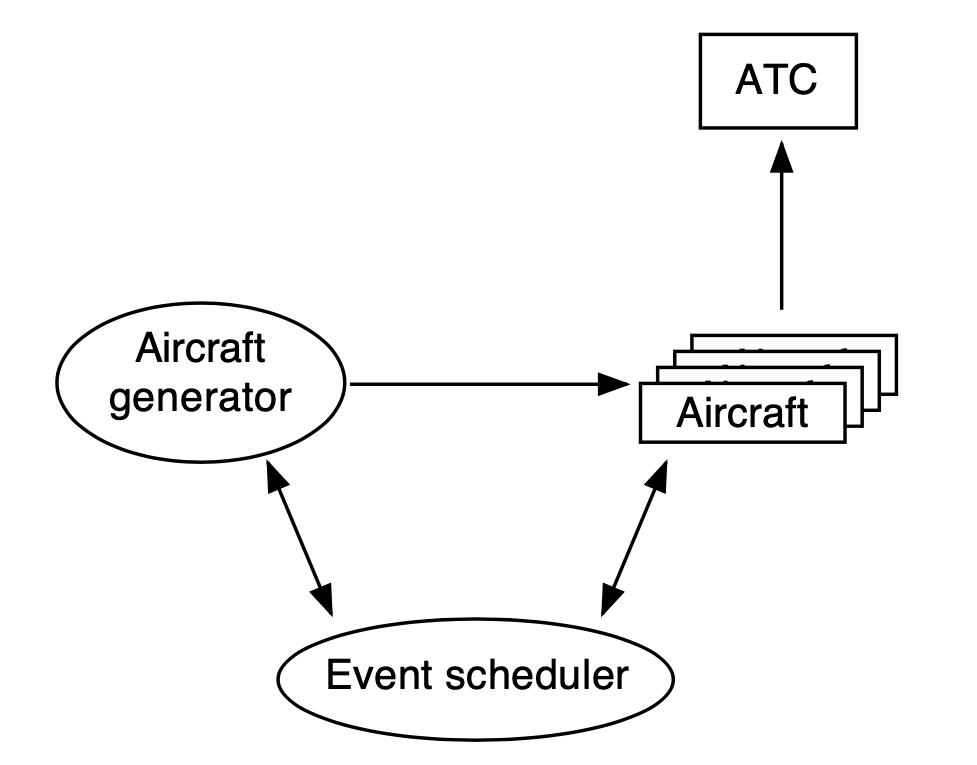
\includegraphics[width=0.9\textwidth]{MathDept-images/Structure.png}
    \end{column}
\end{columns}
\end{frame}


\section{Analysis}
\subsection{Airspace Capacity}
\subsubsection{Setup and Assumptions}
\subsubsection{Data Handling and Processing}
\subsubsection{Simulation results (Round 1)}
\subsection{Avoiding Risk Events}
\subsubsection{Trajectory Algorithm}
\subsubsection{Critical Distances}
\subsubsection{Simulation results (Round 2) improved?}

\begin{frame}[allowframebreaks]{Table of contents}
    \tableofcontents[currentsection, hideothersubsections, subsubsectionstyle=show/show/show/hide]   
\end{frame}
\begin{frame}
\frametitle{Setup and Assumptions}
\vspace{5mm}
- We chose a counting process, \( \{N(t)\} \), with i.i.d waiting times between arrivals sampled from a censored exponential distribution.
\vspace{3mm} \\
- These waiting times, denoted by \( W_1, W_2, \ldots \), are determined as:

\[ W_i = \max(\kappa, U_i), \quad i = 1, 2, \ldots \]

- Here, \( U_1, U_2, \ldots \) are independent and identically exponentially distributed variables with mean $\mu = 90 $ seconds. \vspace{3mm}\\

- We also introduced the constant \( \kappa \) as a control parameter, controlling the flow of traffic into \( \mathcal{A} \). In our simulations, \( \kappa \) varied from 10 to 50 seconds.
\end{frame}
\begin{frame}
\frametitle{Data Handling and Processing}
\vspace{5mm}
\begin{itemize}
    \item All flights through $\mathcal{A}$ are assumed to be either northbound or eastbound.
    \vspace{3mm}
    \item The probability of a flight being northbound is the same as the probability of it being eastbound, which is $\frac{1}{2}$.
    \vspace{3mm}
    \item For northbound flights, arrival points are randomly selected within the interval $I_S$ along the southern border of $\mathcal{A}$, and departure points within the interval $I_N$ along the northern border.
    \vspace{3mm}
    \item For eastbound flights, arrival points are randomly selected within the interval $I_W$ along the western border of $\mathcal{A}$, and departure points within the interval $I_E$ along the eastern border.
\end{itemize}
\end{frame}
\begin{frame}
\frametitle{Simulation results (Round 1)}
\vspace{5mm}
    \centering
    \begin{figure}
    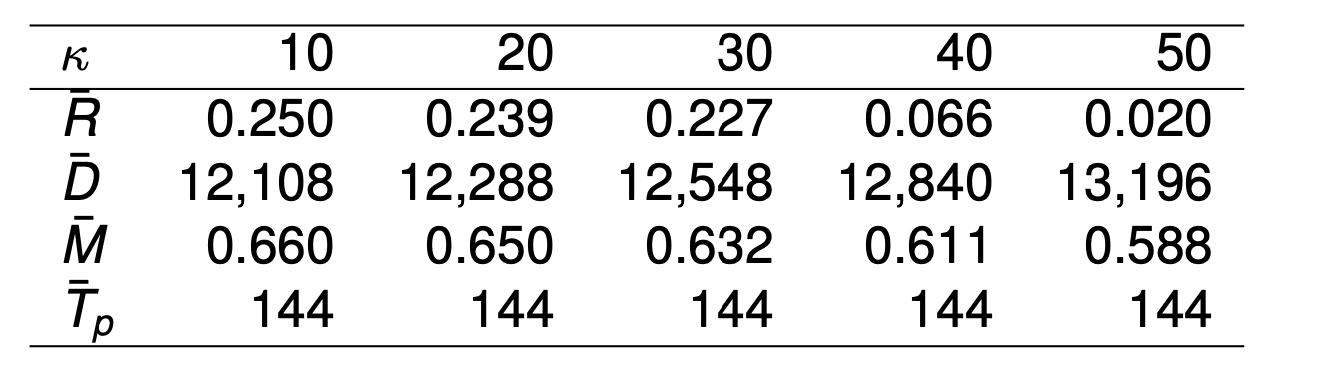
\includegraphics[width=0.9\textwidth]{MathDept-images/simul_risk.png}
    \caption{Estimated criticality and performance measures as a function of the control parameter $\kappa$.}
    \end{figure}
\end{frame}
\begin{frame}
    \frametitle{Avoiding Risk Events}
    \framesubtitle{Trajectory Algorithm}
For each point of time $t$ and for each $j \in J(t)$ do the following:

STEP 1. Calculate the "ideal" velocity for the $j$ th aircraft as:
$$
\dot{\boldsymbol{x}}_j(t)=\frac{\boldsymbol{X}_{d, j}-\boldsymbol{x}_j(t)}{\left\|\boldsymbol{X}_{d, j}-\boldsymbol{x}_j(t)\right\|} s_j .
$$
\pause 
STEP 2. Find the nearest aircraft and adjust the trajectory if needed to avoid a risk event.
\vspace{2mm}\\
\pause
STEP 3a. If no action is needed, use the ideal velocity in the interval $[t, t+d t)$, and update the position: $\boldsymbol{x}_{j}(t + dt) = \boldsymbol{x}_{j}(t) + \dot{\boldsymbol{x}_{j}}dt$ \vspace{2mm}\\
\pause
STEP 3b.If an action is needed, make a “turn”. That is, replace the ideal velocity by:
$$\dot{\boldsymbol{x}}_j^{\prime}(t)=\Lambda \dot{\boldsymbol{x}}_j(t)$$ 
in the interval $[t, t+d t)$ where $\Lambda$ is the $3 \times 3$ horizontal rotation matrix.
\end{frame}
\begin{frame}
\frametitle{Avoiding Risk Events}
\framesubtitle{Trajectory Algorithm cont.}
- To further specify the algorithm:
\begin{enumerate}
    \item We need a criterion for when an action is needed.
    \item We must determine matrix $\Lambda$ based on relative positions and velocities of two aircraft.
\end{enumerate}
- To do this:
\begin{itemize}
    \item Consider \(j\)th aircraft \(a_j\) at time \(t_0\).
    \item Assume \(a_k\) is the closest aircraft to \(a_j\).
    \item Focus on relative positions and velocities of \(a_j\) as seen from \(a_k\), denoted $\boldsymbol{x}_{j,k}(t)$ and $\dot{\boldsymbol{x}}_{j,k}(t)$.
\end{itemize}
Where $\boldsymbol{x}_{j,k}(t)$ and $\dot{\boldsymbol{x}}_{j,k}(t)$ are expressed as follows: 
\begin{align*}
    \boldsymbol{x}_{j,k}(t) &= \boldsymbol{x}_{j}(t) - \boldsymbol{x}_{k}(t) \\[3pt]
    \dot{\boldsymbol{x}}_{j,k}(t) &= \dot{\boldsymbol{x}}_{j}(t) - \dot{\boldsymbol{x}}_{k}(t)
\end{align*}
\end{frame}
\begin{frame}
\frametitle{Avoiding Risk Events}
\framesubtitle{Trajectory Algorithm cont.}
\vspace{3mm}
\begin{itemize}
    \item Distance between \(a_k\) and \(a_j\) at time \(t_0\): \(\left\| \boldsymbol{x}_{j, k} (t_0) \right\|\).
    \item If large, no trajectory modification for \(a_j\) is needed.
    \item Alert distance \(C_A\) introduced to manage this, set \(> C\) to avoid risk events.
    \item In simulations, \(C_A\) set to twice \(C\) (\(5\) nautical miles or \(9,260\) meters).
\end{itemize}
\end{frame}
\begin{frame}
\frametitle{Avoiding Risk Events}
\framesubtitle{Trajectory Algorithm cont.}
\textbf{Case:} \(\left\| \boldsymbol{x}_{j, k} (t_0) \right\| \leq C_A\)
\begin{itemize}
    \item Determine if aircrafts get closer or further apart over time.
    \item Consider distance \(\Delta(t) = \left\| \boldsymbol{x}_{j, k}(t) \right\|\).
    \item Assuming no action:
    \[ \boldsymbol{x}_{j, k}(t) = \boldsymbol{x}_{j, k}(t_0) + \dot{\boldsymbol{x}}_{j, k}(t_0)(t - t_0) \]
    \item Find time \(t_1\) when \(\Delta(t)\) is minimized:
    \[ t_1 = t_0 - \frac{\boldsymbol{x}_{j, k}(t_0)^T \dot{\boldsymbol{x}}_{j, k}(t_0)}{\dot{\boldsymbol{x}}_{j, k}(t_0)^T \dot{\boldsymbol{x}}_{j, k}(t_0)} \]
\end{itemize}
\end{frame}
\begin{frame}
\frametitle{Avoiding Risk Events}
\framesubtitle{Trajectory Algorithm cont.}
\begin{itemize}
    \item \( t_1 > t_0 \) if and only if: \( \boldsymbol{x}_{j, k}(t_0)^T \dot{\boldsymbol{x}}_{j, k}(t_0) < 0 \).
    \item By inserting the expression for \( t_1 \) into the equation for $\boldsymbol{x}_{j, k}(t)$, we find the position where \( a_j \) is closest to \( a_k \):
    \[ \boldsymbol{x}_{j, k}(t_1) = \boldsymbol{x}_{j, k}(t_0) - \dot{\boldsymbol{x}}_{j, k}(t_0) \frac{\boldsymbol{x}_{j, k}(t_0)^T \dot{\boldsymbol{x}}_{j, k}(t_0)}{\dot{\boldsymbol{x}}_{j, k}(t_0)^T \dot{\boldsymbol{x}}_{j, k}(t_0)} \]
    \item If \( t_1 > t_0 \) and \( \Delta(t_1) \leq C \), action is needed to avoid a risk event.
    \item Our approach involves making a "turn" by rotating the velocity vectors by \( \lambda \) radians.
    \item To determine \( \lambda \), we introduce the normal vector to the relative position vector, \( \boldsymbol{y}_{j,k}(t_0) \), obtained by rotating \( \boldsymbol{x}_{j,k}(t_0) \) counterclockwise by \( \pi/2 \) radians.
\end{itemize}
\end{frame}
\begin{frame}
    \frametitle{Avoiding Risk Events}
    \framesubtitle{Trajectory Algorithm cont.}
    \textbf{Case 1:} $\dot{\boldsymbol{x}}_{j, k}(t_0)^T \dot{\boldsymbol{y}}_{j, k}(t_0) > 0$ \\ \textbf{Case 2:} $\dot{\boldsymbol{x}}_{j, k}(t_0)^T \dot{\boldsymbol{y}}_{j, k}(t_0) < 0$ \\
    \textbf{Case 3:} $\dot{\boldsymbol{x}}_{j, k}(t_0)^T \dot{\boldsymbol{y}}_{j, k}(t_0) = 0$
    \begin{figure}
        \centering
        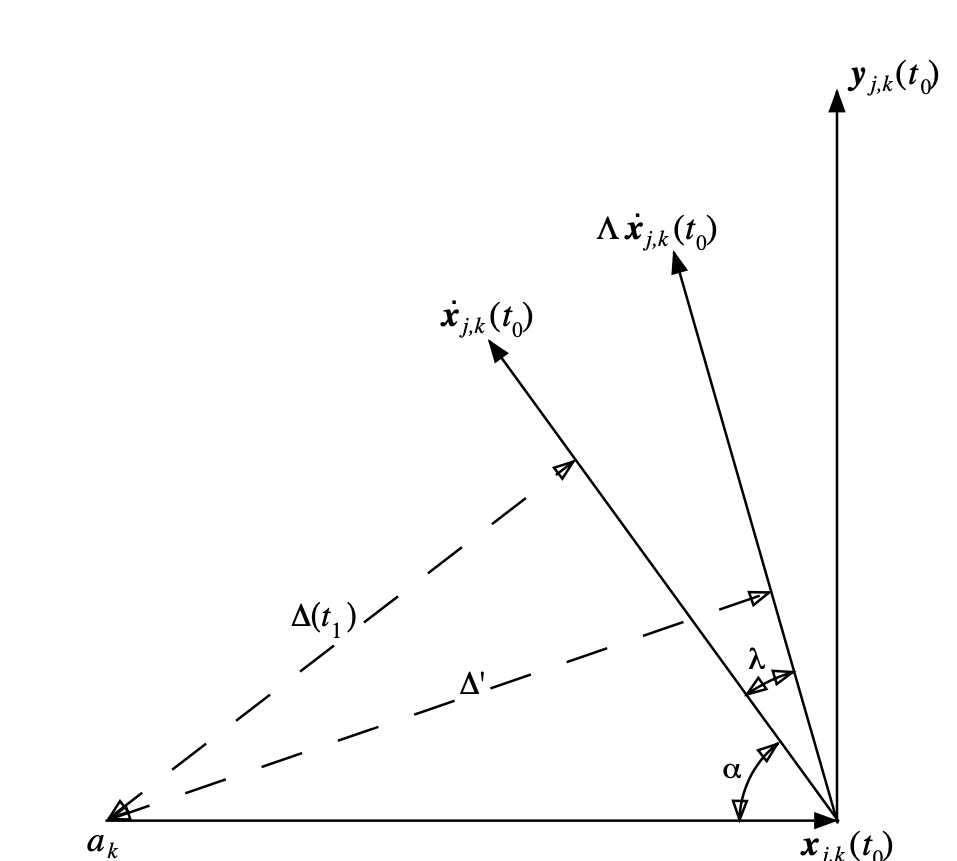
\includegraphics[width=0.4\textwidth]{MathDept-images/rotation_axis.png}
        \caption{Rotating the relative velocity}
    \end{figure}
\end{frame}

\begin{frame}
\frametitle{Avoiding Risk Events}
\framesubtitle{Simulation results (Round 2)}
\begin{columns}[T]
\begin{column}{0.5\textwidth}
\centering
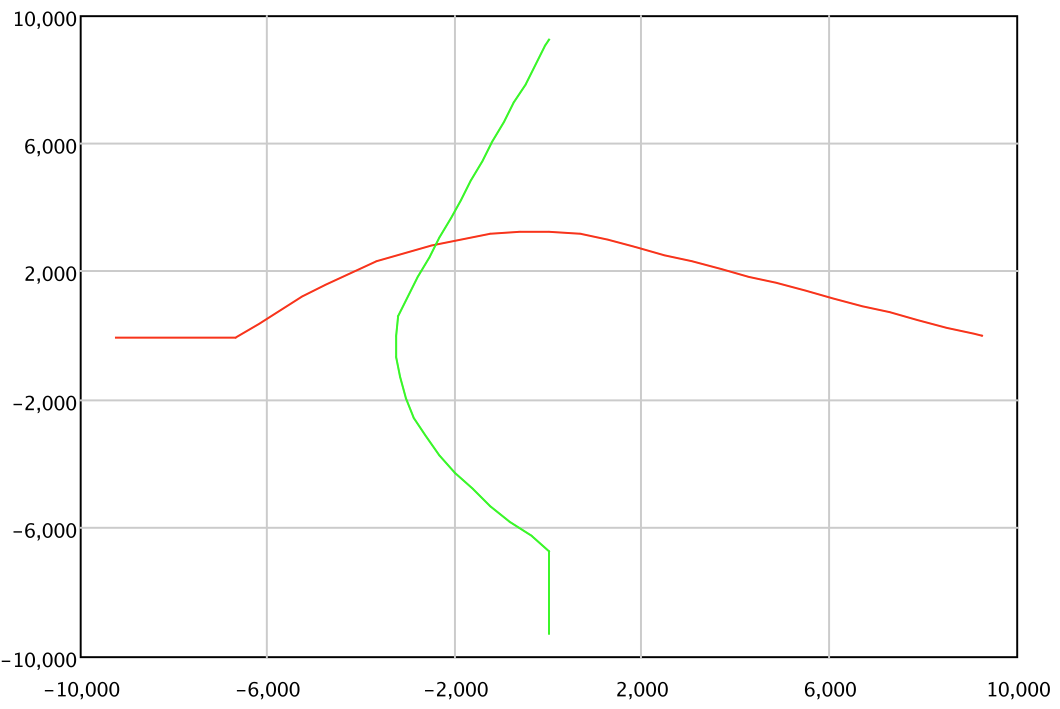
\includegraphics[width=\textwidth]{MathDept-images/Rotation_trajc.png}
\end{column}
\begin{column}{0.53\textwidth}
\centering
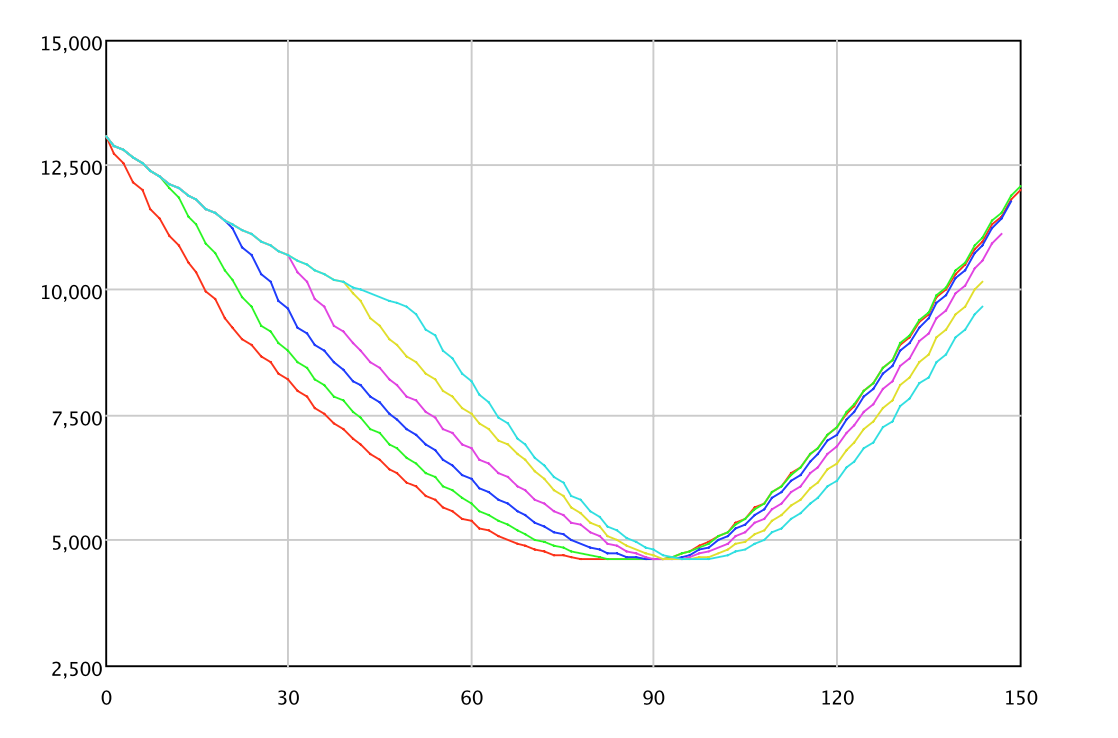
\includegraphics[width=\textwidth]{MathDept-images/flight_dist.png}
\end{column}
\end{columns}
\begin{itemize}
    \item \textbf{Plot left}: Trajectories of two flights 
    \item \textbf{Plot right}: Distance (meters) between flights as a function of time
\end{itemize}
\end{frame}
\begin{frame}
\frametitle{Avoiding Risk Events}
\framesubtitle{Simulation results (Round 2)}
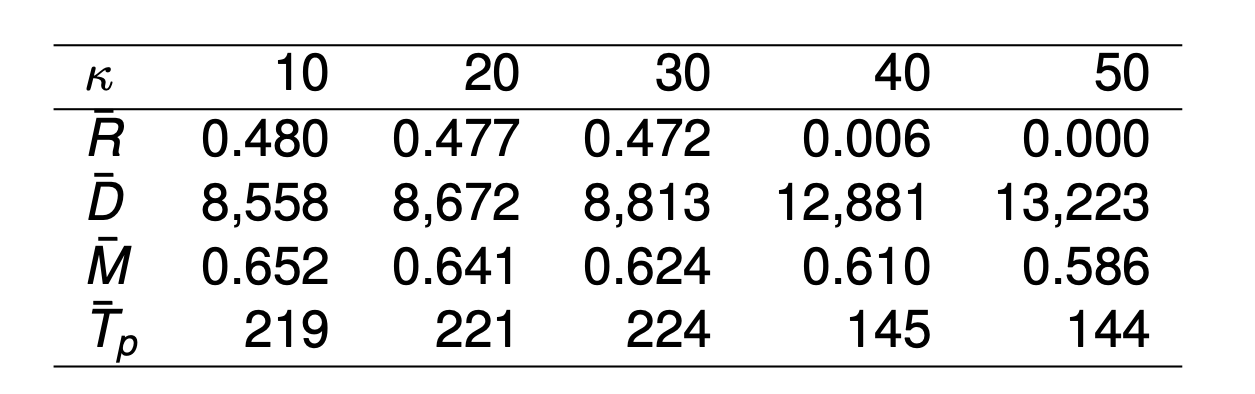
\includegraphics[width=\textwidth]{MathDept-images/simul_risk_av.png}
\pause 
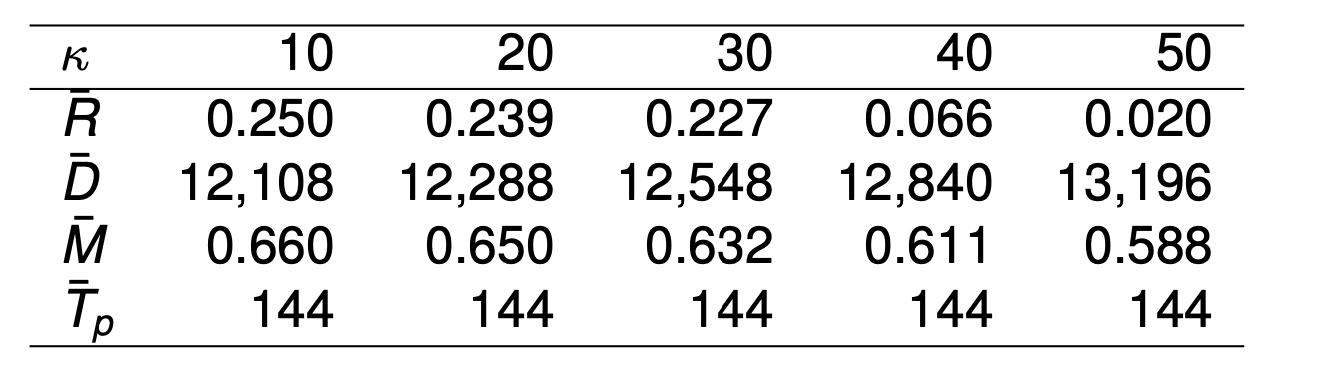
\includegraphics[width=\textwidth]{MathDept-images/simul_risk.png}
\end{frame}
\begin{frame}
\begin{columns}[T]
\begin{column}{0.5\textwidth}
\centering
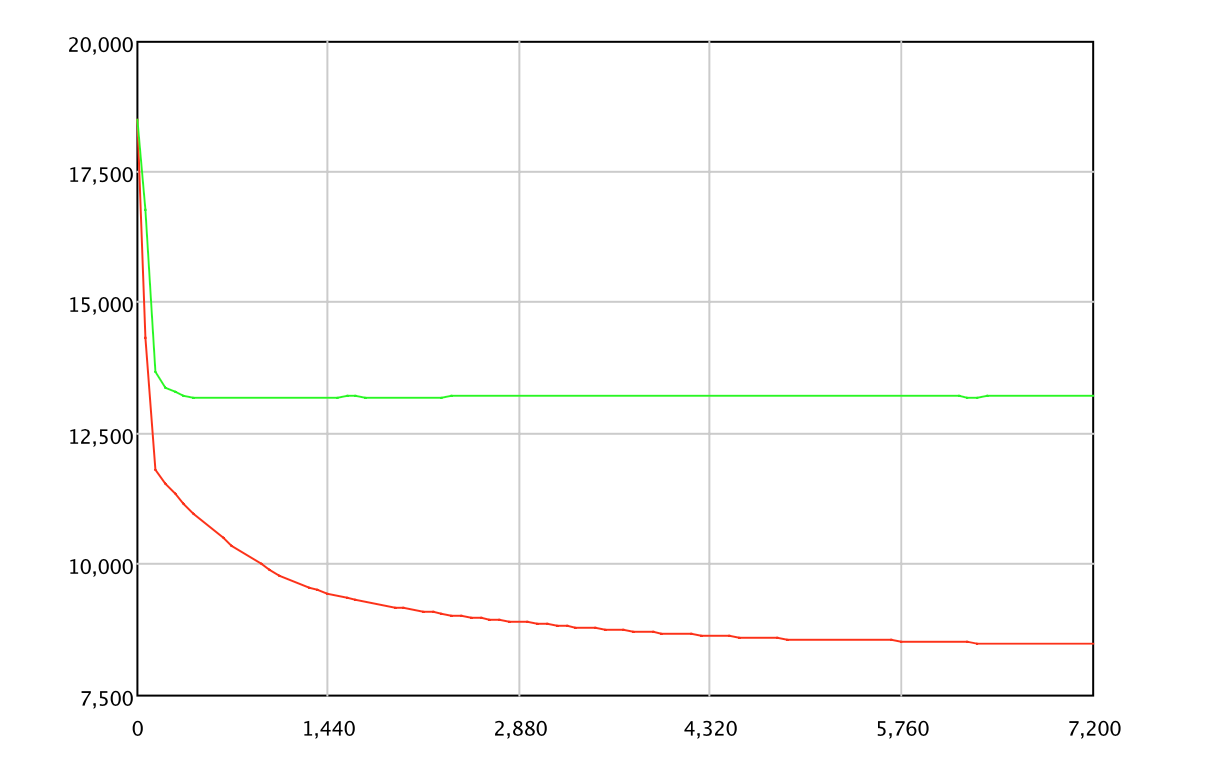
\includegraphics[width=\textwidth]{MathDept-images/distance_simul.png}
\end{column}
\begin{column}{0.5\textwidth}
\centering
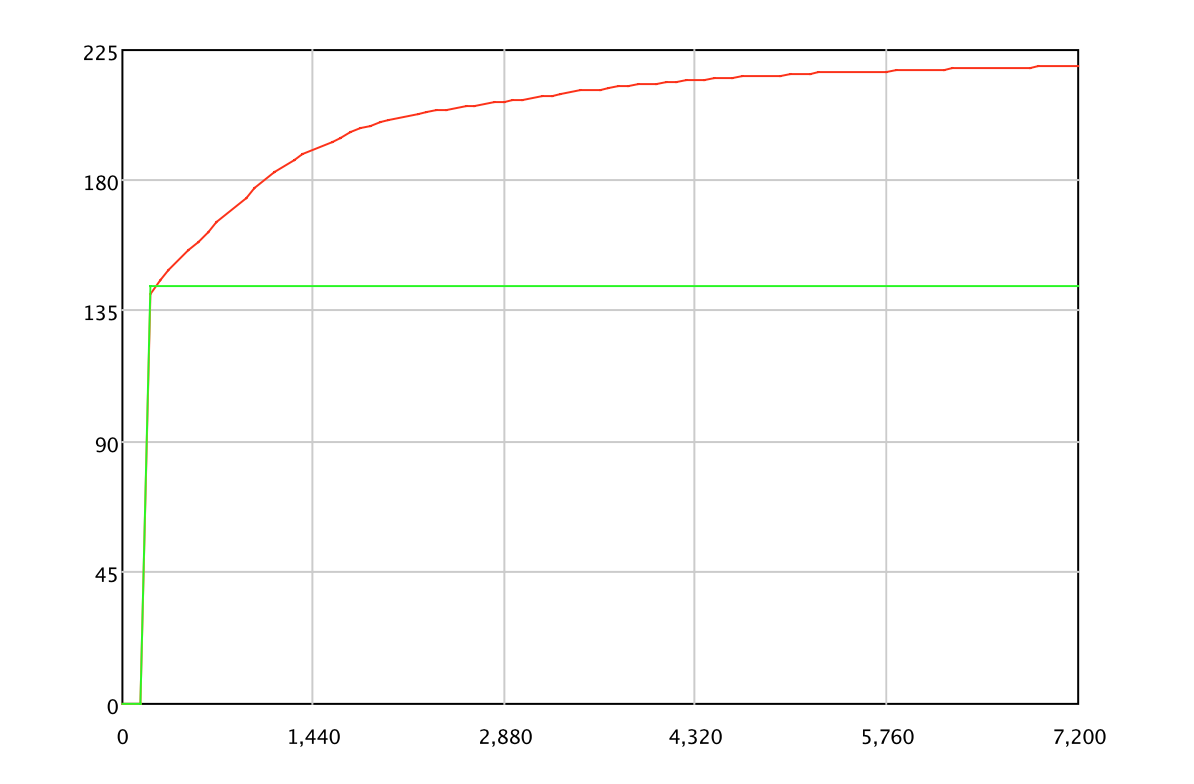
\includegraphics[width=\textwidth]{MathDept-images/number_process.png}
\end{column}
\end{columns}
\begin{itemize}
    \item \textbf{Plot left}: Average minimum flight distances (meters) as functions of time for $\kappa = 10$ (lower curve) and $\kappa = 50$ (upper curve)
    \item \textbf{Plot right}: Average processing times as functions of time for $\kappa = 10$ (lower curve) and $\kappa = 50$ (upper curve)
\end{itemize}
\end{frame}
\section{Conclusion}
\begin{frame}[allowframebreaks]{Table of contents}
    \tableofcontents[currentsection,hideothersubsections, subsubsectionstyle=show/show/show/hide]   
\end{frame}
\begin{frame}{Conclusion}
\frametitle{Summary}
\begin{enumerate}
    \item We have demonstrated how to create hybrid simulation models for aircraft paths in a random environment.
    \item Examined two related concerns with the model:
    \begin{itemize}
        \item Organizing the arrival process
        \item Preventing situations/events of risk by adjusting paths dynamically
    \end{itemize}
    \item It's essential to study both issues together within a unified model.
    \item Future work:
    \begin{itemize}
        \item Enhancing and refining the models and algorithms
        \item Modeling smoother aircraft movements (in three dimensions)
        \item Incorporating other random factors such as weather
    \end{itemize}
\end{enumerate}
\end{frame}
\section{References}


\begin{frame}[allowframebreaks]
\frametitle{References}
\nocite{*}
\bibliographystyle{plain}
\bibliography{references} % Include the bibliography file
\end{frame}


\end{document}